\graphicspath{{chapters/greco/images/level4/}}

\subsection{GRECO Level 4 Cuts}
The first GRECO-specific cut level, designated \emph{level 4}, or \emph{L4}, was first introduced in 2011 using variables common to higher energy cascade analyses within IceCube. 

At the start of this series of cuts is requirement of at least three hit DOMs in the hit series associated with an event. 
This is an extremely loose cut, required solely for the successful processing of other cuts.

The remaining cuts at L4 can be divided into two groups: those that rely on a rough reconstruction of the event and those that are based solely on charge deposition.

\subsubsection{FirstHit Z}
\begin{figure}[h]
	\centering
		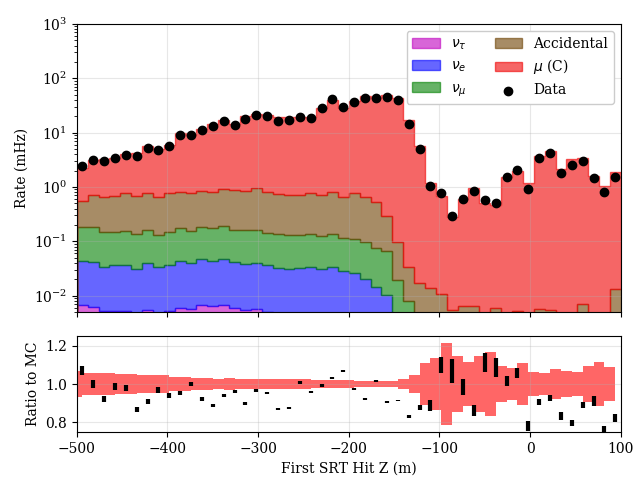
\includegraphics[width=2.5in]{FirstHitZ_log.png}
		\caption[The FirstHit Z position]{The Z position of the first hit in a cleaned hit series. Note the shape difference between the atmospheric muons in red and the various neutrino flavors, particularly above -200 meters.}
	\label{fig:firsthitz_log}
\end{figure}

Muons generated in the upper atmosphere through cosmic ray air showers will generally be visible as they enter the detector. 
As they pass through the veto layers, the muons may emit light via Cherenkov emission or via stochastic processes. 
This light leaves a signature behind in the detector in the form of hits along the true muon track. 

Because the muon tracks are primarily steeply inclined, most will leave hits in the upper part of the detector.
Neutrinos, on the other hand, will emit light following an interaction.
For the low-energy neutrinos of interest to this analysis, interactions will occur primarily in the DeepCore fiducial region, leading to little or no light emission in the top half of the detector. 
This difference between neutrino and muon emission in the upper part of the detector can be used to identify background muons with little additional processing.
For this analysis, the first hit in a cleaned hit series, the time-window cleaned DeepCore pulses, is called the \emph{FirstHit Z} in the Level 4 cuts.

\subsubsection{NAbove200}
\begin{figure}[h]
	\centering
		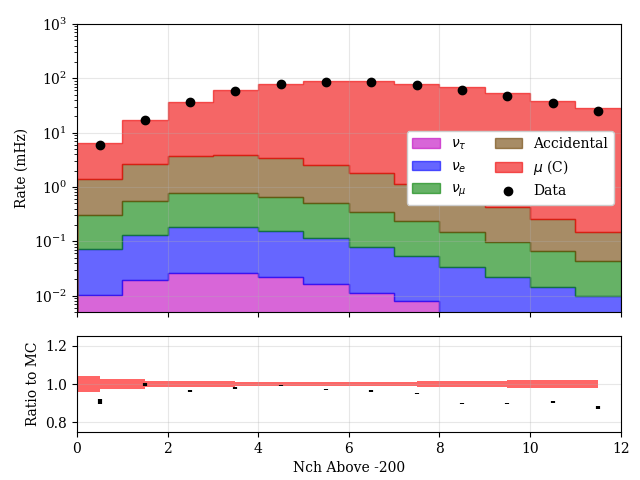
\includegraphics[width=2.5in]{NAbove200_log.png}
		\caption[Number of Hits Above Z=-200]{The number of hits above Z=-200 meters}
	\label{fig:nabove200_log}
\end{figure}

The position of the first hit in DeepCore is not the only low-level cut to arise from the emissions of the muon and neutrinos. 
The total charge of recorded hits occuring in the top of the detector is also used in the analysis. 
This variable, known as \emph{NAbove200}, counts the amount of charge occuring before the SMT3 trigger above a depth of -200 meters.

\subsubsection{QR6/C2QR6}
\begin{figure}{h}%
	\centering
		\subfloat[QR6]{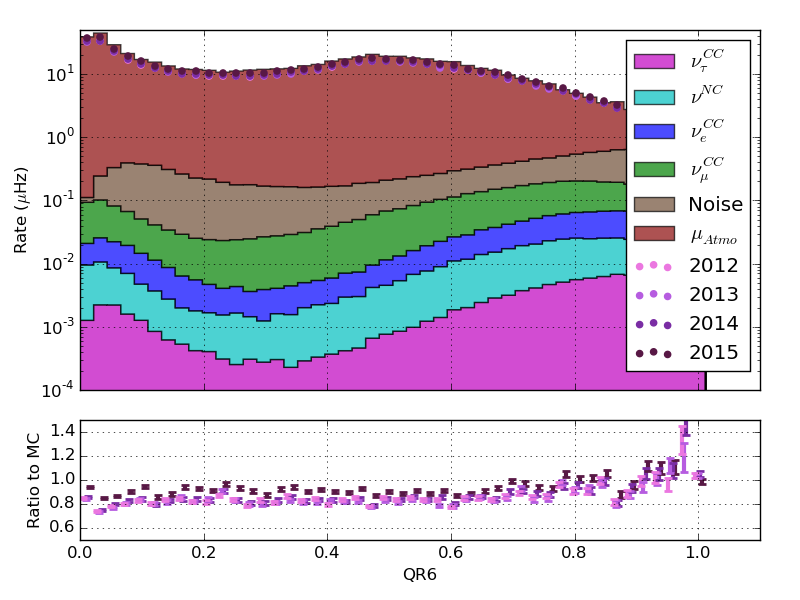
\includegraphics[width=2.3in]{QR6_log.png}}%
		\subfloat[C2QR6]{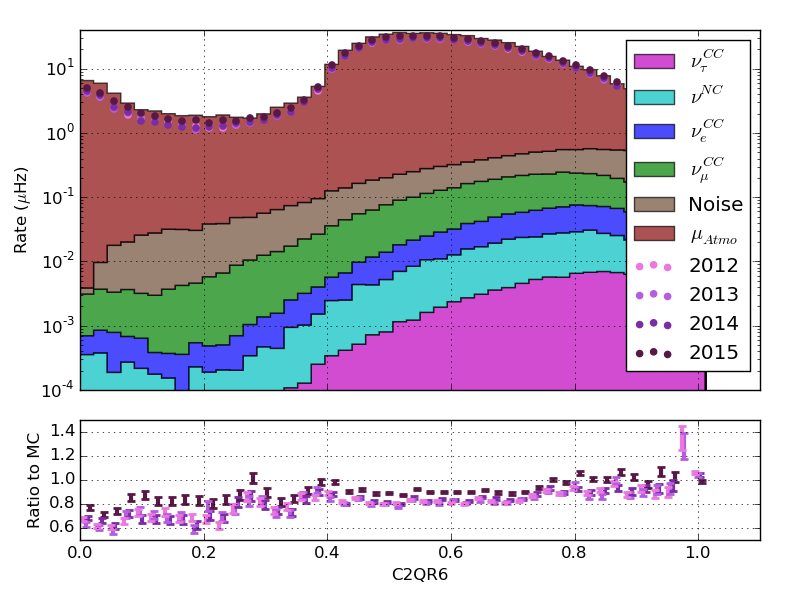
\includegraphics[width=2.3in]{C2QR6_log.png}}%
	\caption[QR6 and C2QR6]{The charge ratio variables used in the L4 cuts.}%
	\label{fig:QR6_and_C2QR6}%
\end{figure}

After a particle interacts, the light emission as a function of time will depend on the type of particle emitting.
A very basic model of cascade-like events assumes that photons are emitted roughly instantaneously from a point-like source at the interaction vertex. 
The photons then travel outward according to a random walk with absorption, leading to a decay in the observed number of photons over time.
A muon, however, acts as an extended source and will emit at multiple points along the muon track until it either falls below the Cherenkov threshold or is stopped.

The light emission is, therefore, more likely to be "peaked" in time for neutrinos than for muons. 
Using this information, two variables are designed to seach for this peakedness in the light detection over time.

The first of these, the \emph{charge-ratio within 600 ns} (hereafter \emph{QR6}), is the ratio of the charge occuring within 600 ns of the first hit compared to the total charge of the event.
The value of 600 ns was chosen in a previous analysis and is not re-optimized here.
Regardless, this time corresponds to roughly two ATWD time windows or approximately 180 meters at the speed of light in vacuum.
This distance, which will correspond to a wide swath of the DeepCore fiducial volume, provides some separation between muons and neutrinos.

\subsubsection{QR6 plot}

Neutrinos and muons do not produce the only hits observed in the detector, however. 
Random detector noise, in particular, can significantly change the choice of time used.
In order to check the effect of random noise contributing the first few hits of the event, a second variable, known as \emph{C2QR6}, is introduced.
This variable is calculated in an identical way to QR6, but the first two observed hits are ignored.

\emph{C2QR6 plot}


\subsubsection{Tensor of Inertia}
\begin{figure}[h]
	\centering
		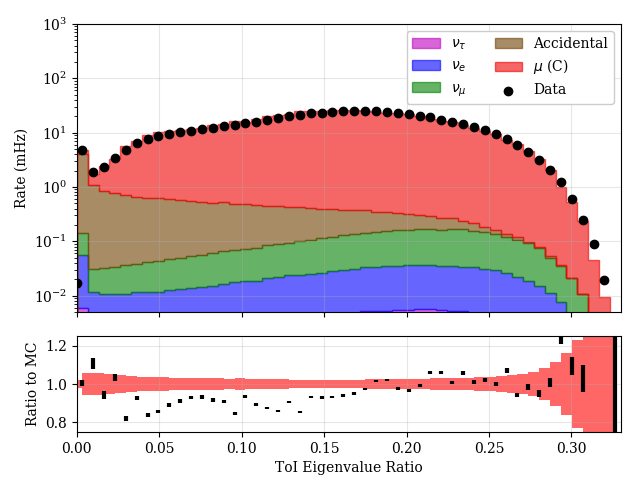
\includegraphics[width=2.5in]{ToIEval_log.png}
		\caption[Tensor-of-Inertia Eigenvalue Ratio]{The eigenvalue ratio from a ToI calculation. Larger values indicate more apparent elongation in the event.}
	\label{fig:toi_log}
\end{figure}

At this early level, the shape difference in the observed hit pattern will be relatively clear.
Neutrinos with energies in the range of 1-100 GeV will appear to be rather small and compact, while muons will have a longer extent in one direction along the muon track than perpendicular to it.
In order to utilize the shape differences between these two types of particles, the \emph{Tensor of Inertia eigenvalue ratio} (more briefly, \emph{ToI}) is used.
This variable is defined in a similar way to the tensor of inertia from mechanics, with the measured charge taking the place of the mass.

\begin{eqnarray}
	I_{X} = \sum_{i=0}^{nhits}(y_i^2 + z_i^2)q_i	
	I_{Y} = \sum_{i=0}^{nhits}(x_i^2 + z_i^2)q_i
	I_{Z} = \sum_{i=0}^{nhits}(x_i^2 + y_i^2)q_i
\end{eqnarray}

These three moments yield information about the shape of the event.
The eigenvalue ratio is defined as 

\begin{equation}
	e = \frac{\mathtt{max}_j(I_j)}{I_{x}+I_{y}+I_{z}}
\end{equation}


\subsubsection{Improved Linefit Speed}
\begin{figure}[h]
	\centering
		\includegraphics[width=2.5in]{iLineFit_Log.png}
		\caption[The improvedLineFit Speed]{The apparent speed, in units of meters per nanosecond, corresponding to the hits in the event. Faster speeds are associated with particle travel instead of light travel.}
	\label{fig:ilinefit_log}
\end{figure}



\subsubsection{The L4 BDT}
\begin{figure}[h]
	\centering
		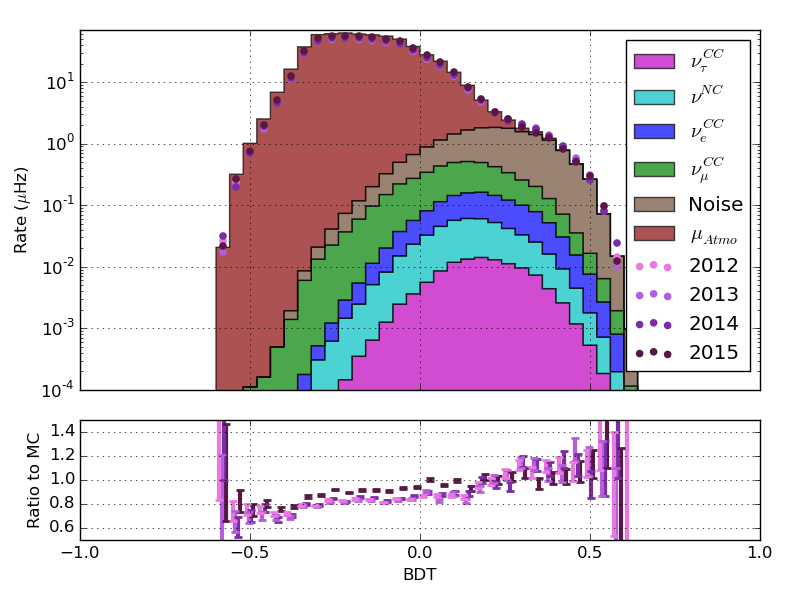
\includegraphics[width=4in]{BDT_log.png}
		\caption[The L4 BDT Score]{The distribution of the boosted decision tree used at L4. A cut is applied at 0.04 to remove a significant fraction of atmospheric muon background events. Note the ratio, which shows disagreement in the very muon-like region. The region of disagreement is removed by the cut.}
	\label{fig:L4_bdt_log}
\end{figure}

A Boosted Decision Tree (\emph{BDT}) is trained at L4 to further reduce the atmospheric muon background by a factor of 10x. 

The variables described above were provided to a BDT training using the CORSIKA 7437 and IceSim3 GENIE simulation. 

Burn sample distributions match in the years 2012/3/4/5, but are notably different for 2011. 
I believe the reason is related to the deployment: once new DOMs are deployed, they take 1-2 years to completely cool down 2011 is therefore excluded for this analysis.

Comparisons to MC show mild disagreement, particularly in the most muon-like regions that get cut away. 
Its not obvious what is the cause of the disagreement, although its possible that the assumed cosmic ray flux model (H4a) is simply an inaccurate model of some part of the spectrum that contributes. 
This may be particularly true, since H3a and H4a contain different compositions at high energies. 
These differences would contribute to different parts of the atmospheric muon spectrum at the detector, where the highest energy atmospheric interactions leading to visible muons will occur at the horizon. 
If these (or other systematics on the CR/muon spectra) give rise to different HE muon distributions, those muons would appear to have clear tracks and would show up on the far left of the BDT distribution.

In the right side of the plot, a shoulder attributable to the noise triggers is visible. 
While this is initially surprising, the reason for this is obvious: the BDT was originally trained with CORSIKA set 7437 and weighted GENIE sets.
Both cases had incorrect modeling of the detector. 
Both had DOM oversizing applied and DOM efficiency set to 0.9 (the old nominal value) instead of the 0.99 that we now use. 
The training itself lacked any pure noise triggers as a reference, and so the BDT picked the most obvious feature of the GENIE sets: that the signal events were primarily low energy with lower light deposition than the background. 
These are also key features of the noise triggers. 
